%%%%%%%%%%%%%%%%%%%%%%%%%%%%%%%%%%%%%%%%%%%%%%%%%%%%%%%%%%%%%%%%%%%%%%
% How to use writeLaTeX:
%
% You edit the source code here on the left, and the preview on the
% right shows you the result within a few seconds.
%
% Bookmark this page and share the URL with your co-authors. They can
% edit at the same time!
%
% You can upload figures, bibliographies, custom classes and
% styles using the files menu.
%
%%%%%%%%%%%%%%%%%%%%%%%%%%%%%%%%%%%%%%%%%%%%%%%%%%%%%%%%%%%%%%%%%%%%%%

\documentclass[12pt]{article}

\usepackage{sbc-template}

\usepackage{graphicx,url}

%\usepackage[brazil]{babel}
\usepackage[utf8]{inputenc}


\sloppy

\title{Implantação ágil no desenvolvimento de software, uma revisão sistemática}

\author{Thiago  de Souza Fonseca Ribeiro\inst{1}}


\address{UnB -- Universidade de Brasília -- Campus Gama -- FGA
  \email{thiagovsk@aluno.unb.br}
}

\begin{document}

\maketitle

\begin{abstract}
  This meta-paper describes the style to be used in articles and short papers
  for SBC conferences. For papers in English, you should add just an abstract
  while for the papers in Portuguese, we also ask for an abstract in
  Portuguese (``resumo''). In both cases, abstracts should not have more than
  10 lines and must be in the first page of the paper.
\end{abstract}

\begin{resumo}
  Este meta-artigo descreve o estilo a ser usado na confecção de artigos e
  resumos de artigos para publicação nos anais das conferências organizadas
  pela SBC. É solicitada a escrita de resumo e abstract apenas para os artigos
  escritos em português. Artigos em inglês deverão apresentar apenas abstract.
  Nos dois casos, o autor deve tomar cuidado para que o resumo (e o abstract)
  não ultrapassem 10 linhas cada, sendo que ambos devem estar na primeira
  página do artigos.
\end{resumo}

\section{Introdução}\label{sec1}

Os métodos ágeis de desenvolvimento de software têm sido
cada vez mais adotados em todo o mundo e se tornaram uma das correntes no desenvolvimento de software como um todo. Os métodos ágeis também tiveram um impacto sobre a educação em engenharia de software nas universidades que começaram a adaptar os seus cursos para acomodar esta nova forma de desenvolvimento de software. \cite{brazil}.

O desenvolvimento de software de forma ágil e traz como necessidade se adapatar a mudanças do mercado e as necessidades do cliente, com a pressão de colocar um produto no mercado no menor espaço de tempo possível, pois um atraso pode acarretar na perda de clientes ao disponibilizar novas funcionalidades de um software. Para resolver esta situação, práticas ágeis têm aumentado a capacidade em que as empresas têm de desenvolvimento de software, e que assim consigam lidar com a complexa mudança de requisitos e a grande variedade das necessidades do mercado \cite{dzamashvili2010impact}.

Entretando software só oferece valor para os clientes quando eles estão implantados em produção e que possam proporcionar as funcionalidades para o usuário final. \cite{6612879} Com isso, a implantação de um software não pode ser um processo lento, já que quanto mais rápido o software é disponibilizado para os seus usuários mais rápido a equipe de desenvolvimento consegue colher o feedback desses usuários.

Com a popularização do desenvolvimento ágil, bem com o acesso barato a recursos de hardware como virtualização e computação em nuvem, contribuiram para a evolução do processo de entrega de software, tornando mais rápido e acessível para as empresas a lançarem seu software continuamente \cite{6612879}.

De acordo com \cite{6449236} a escolha da metodologia de desenvolvimento pode impactar no tempo de entrega de um software, um exemplo de comparação é feito com as metodologias e o próprio facebook:

\begin{itemize}
  \item \textbf{Waterfall ou Processo Cascata:} Uma única bez
    \item \textbf{Desenvolvimento Evolutivo:} EM meses
    \item \textbf{Desenvolvimento ágil:} Em semanas
    \item \textbf{Facebook:} Em dias
    \item \textbf{Implantação contínua:} Em horas
\end{itemize}


No contexto do modelo cascata, o objetivo final é entregar o produto de software no fim do projeto, dentro do contexto de desenvolvimento ágil ou sistemas evolutivos tais como Linux, as entregas são periódicas \cite{6612879}. Mas as práticas que as empresas de Internet usam é conhecido como implantação contínua, isso vêm da necessidade de colher o rapidamente  o feedback do usuário final, e isso reflete o hábito de implantar um novo código com uma série de pequenas alterações no momento em que ele está pronto.

Contudo,enquanto métodos e práticas ágeis são atraentes para muitos software nas empresas de desenvolvimento, existem poucas empresas (por exemplo, Facebook, IBM, Adobe e Microsoft que tiveram sucesso na implementação de práticas ágeis para implantação contínua de software. \cite{Claps201521}. Porém de acordo com \cite{6265084} a complexidade dos sistemas voltado para a Internet têm aumentado,no passado a maioria das aplicações de softwares eram pequenas aplicações simples que podem ser instalados numa ambiente padrão básico, porém atualmente os sistemas voltado para a internet consistem em várias aplicações que precisam ser integradas, o que torna o processo de implantção cada vez mais complexo. \cite{6265084}

A forma como as empresas devem entregar software vai por meio de uma onda de mudanças, necessidades do mercado estão mudando continuamente, as tecnologias estão mudando rapidamente, existe mais pressão para se adaptar ao mercado e a necessidade de entregar rapidamente devido a competitividade do mercado. As empresas não podem já não se dar ao luxo de deixar o cliente à espera de 6 meses ou 1 ano para o lançamento de uma nova versão e, em seguida, solicitar feedback de cliente sobre como software se comporta. Os clientes esperam que o desenvolvimento seja contínuo de modo que eles podem fornecer um feedback rápido.

A fim de enfrentar os desafios de hoje, as empresas precisam ser  ágeis em todas as fases de ciclo de vida de desenvolvimento de um software. Ao longo dos anos as organizações adotaram muitos processos otimizações em seu desenvolvimento ágil. No entanto,nessa evolução tem sido deixando de lado a operações de entrega de software \cite{7173368}. Com isso surge um movimento dentro do desenvolvimento ágil de software conhecido com implantação contínua de software, que propõe evoluir o processo de entrega de software, tornando-o mais rápido e objetivo.

\section{Implantação Contínua de Software} \label{sec2}

Implantação contínua de software é um processo de engenharia de software que foca na entrega rápida de mudanças de software para os usuários finais\cite{7284592}, e neste processo gradual as alterações no software são automaticamente testadas, e frequentemente enviadas para ambientes de teste e produção.

Implantação contínua também tem importantes benefícios do ponto de vista de produção de software. Implantações freqüentes implica que cada implantação introduz apenas uma quantidade limitada de novo código. Isto reduz (mas não elimina) o risco de que algo vai dar errado \cite{6449236}. A capacidade para implantar código rapidamente e em pequenos incrementos sem medo permite uma rápida inovação. Outro benefício das implantações pequenas e rápidas  é que podemos facilmente identificar a origem de bugs: eles são mais prováveveis de aparecer nas mudanças mais recentes, e sua implementação ainda está fresca na mente dos engenheiros.

As empresas de software que estão usando a implantação contínua
relataram vários benefícios deste processo de software, tais como
maior satisfação do cliente, a melhoria da qualidade do software,
e economias no esforço de desenvolvimento \cite{7057604}. Apesar de ser um processo de software emergente que proporciona vários benefícios, profissionais de software têm identificado a falta de
compreensão de implantação contínua sendo ela um grande desafio. Grandes empresas estão usando implantação contínua para implantar o seu produto \cite{7284592} como por exemplo:

\begin{itemize}
  \item Facebook
    \item Google
  \item Github
    \item Amazon
    \item Facebook
\end{itemize}

\subsection{Devops} \label{sec2:sub1}

Um dos problemas encontrados nas empresas é que depois que os desenvolvedores terminavam as funcionalidades, o código era entregue a uma equipe de implantação, que ficaria responsável por implantar aquele código nos servidores de teste e produção, e muitas vezes essa equipe não tinha conhecimento das implementações e isso poderia acarretar em problemas e atraso na implantação. Com isso nasceu o DevOps que é uma peça fundamental de otimização da entrega de software. Opiniões têm mostrado que, em maioria das organizações operações lado de entrega é significativa contribuinte para o atraso na entrega de software. DevOps recomenda automatizar a implantação de software e provisionamento de hardware. \cite{7173368}

DevOps é um conjunto de princípios para a entrega de software onde foco é a velocidade de entrega, teste contínuo , feedback contínuo e a capacidade de reagir a mudam mais rapidamente \cite{7173368}. DevOps estende os princípios ágeis para todo o funil da entrega de entrega de software, onde o time de desenvolvimento entrega várias construções com funcionalidades novas enquanto a equipe de operações organiza nas implantações.

\begin{figure}[ht]
\centering
\includegraphics[width=.5\textwidth]{Captura_de_tela_de_2015-11-11_23-38-31.png}
\caption{O gargalo de implantação de software - Retirado de \cite{7173368}}
\label{fig:exampleFig1}
\end{figure}

DevOps também é um conjunto de práticas que defendem a colaboração entre desenvolvedores de software e operações de TI onde o objetivo é
encurtar o ciclo de feedback, e isso se encaixa dentro de contexto de implantação contínua. Conforme Huttermann \cite{httermann2012devops}, DevOps enfatiza a capacitação de pessoas mais do que processos, também a necessidade de automação no desenvolvimento de novo software, que institui medidas de qualidade e criar uma cultura de partilha de conhecimento entre as pessoas.A comunidade DevOps defende a comunicação entre a equipe de operações e a equipe de desenvolvimento como um meio de assegurar que o os desenvolvedores entenderem os problemas associados com as operações. Um dos principais benefícios da DevOps é a capacidade de quantificar aspectos do desenvolvimento, isto é, levar à melhoria do desenvolvimento do produto, devido à um foco mais nítido em agilidade das entregas.

Quando as equipes de desenvolvimento e operações passam a trabalhar juntos em uma so equipe DevOps, os desenvolvedores compreendem a dificuldade de implantação de softwre quando não existe uma certa cadência no desenvolvimento, com isso a equipe de DevOps deve coordenar tais atividades através de vários processos de desenvolvimento ágil como implantação contínua e testes automatizados \cite{6265084}.

Um grande facilitador do DevOps são as ferramentas de gerenciamento de configuração. Tais ferramentas permitem controlar e automatizar a configuração de todos os elementos que compõem uma aplicação, são elas: softwares previamente instalados, usuários, serviços em execução, arquivos de configuração,tarefas programadas, configurações de rede, armazenamento, monitoramento e segurança. \cite{6265084}. Existem também Ferramentas populares como Puppet e Chef, e sua função principal é automatizar a configuração de um sistema. É possível escrever algumas regras que expressam como um código de software deve ser configurado, e a ferramenta irá configurar o sistema em conformidade com o que foi escrito. Você pode usar o tais  ferramentas para configurar um novo sistema para adicionar novas funcionalidades ou até mesmo para reparar um sistema.

\section{Metodologia: Planejamento da Revisão Sistemática} \label{sec3}

Segundo Kitchenham \cite{kitchenham2004procedures} a maior parte das pesquisas começa com uma revisão de literatura, no entanto, para ter valor científico é necessário que essa revisão seja feita de forma abrangente, não tendenciosa, aberta e objetiva. Por isso a necessidade de utilizar a revisão sistemática, que deve identificar, interpretar e avaliar todas as pesquisas disponíveis e relevantes sobre uma questão \cite{keele2007guidelines}. Para isso a revisão sistemática segue um protocolo de busca, que deve conter todas as informações que permitam que a revisão seja repetida por outros pesquisadores interessados no trabalho desenvolvido.

De acordo com \cite{brereton2007lessons} a revisão sistemática envolve três fases, resumidamente as fases são: Planejamento, Execução e análise dos resultados. Neste trabalho cada faze aborda:

 \begin{itemize}
   \item  \textbf{Planejamento: } Identificação  das  necessidades  para  a  revisão  e  elaboração do protocolo, o protocolo que deverá orientar toda a revisão sistemática. Nele deve conter as informações sobre o objetivo, a descrição do problema, as questões
da pesquisa e os métodos e critérios utilizados para a busca, seleção, avaliação e extração de dados.
   \item  \textbf{Execução: } Na fase de execução, os métodos descritos no protocolo são aplicados e documentados, além da identificação da pesquisa, seleção e avaliação da qualidade  dos  estudos.
      \item  \textbf{Análise dos Resultados: }Na fase de análise dos resultados os dados dos estudos são extraídos e sintetizados e os
resultados são analisados.
 \end{itemize}

\subsection{Objetivos} \label{sec3:subsec1}

O objetivo deste trabalho foi identificar como é feito o processo de implantção de software em equipes de desenvolvimento que utilizam métodos ágeis, identificando quais os procedimentos e técnicas utilizadas nos trabalhos relacionados, a partir de publicações científicas ou estudos primários.

\subsection{Questão de Pesquisa} \label{sec3:subsec2}

A partir do objetivo estabelecido na Seção \ref{sec3:subsec1}, foi elaborada a seguinte questão de pesquisa:

 \begin{itemize}
   \item  \textbf{Questão de Pesquisa: Quais são as formas de otimizar o processo de implantação de software utilizadas em equipes que trabalham utilizando métodos ágeis? }
 \end{itemize}

Essas questões deverão ser respondidas ao final da revisão sistemática.

\subsection{Métodos de Busca de Publicações} \label{sec3:subsec3}

Esta  Subseção  descreve  onde  e  como  foram  realizadas
as  buscas  desta  pesquisa. Apresentam-se também as palavras-chave utilizadas para a geração da string  de busca e os idiomas aceitos para a seleção dos resultados.

As fontes selecionadas para realização deste trabalho foram pesquisadas nas bases eletrônicas de dados disponíveis no portal CAPES, incluindo documentos indexados nas seguintes bases:

 \begin{itemize}
   \item  \textbf{Periódicos CAPES}
   \item  \textbf{IEEEXplore}
   \item  \textbf{Springer}
 \end{itemize}

As seguintes palavras foram utilizadas para fazer as buscas de estudos:

 \begin{itemize}
   \item  \textbf{Agile}
   \item  \textbf{Process Software Deployment}
   \item  \textbf{Devops}
   \item  \textbf{Continuous Delivery}
   \item  \textbf{Continuous Deploy}

 \end{itemize}

Com o intuito de abordar as palavras chave anteriormente definidas, foram definidas as seguitnes strings de busca:

 \begin{itemize}
   \item  \textbf{("deploy" OR "deployment") AND  "agile" AND "software" AND ("devops" OR "continuous delivery" OR "continuous deploy") }
 \end{itemize}

É importante ressaltar que a strings de busca deverá na medida do possível ser igual em todas as máquinas de busca, contudo poderá existir adaptações mas levando em consideração que a string adaptada deverá ser logicamente equivalente a string original.

O idioma escolhido foi o Inglês, também considerou-se qualquer tipo de trabalho ou artigo que fizesse abordagem sobre características de implantação de software no contexto de métodos ágeis.

\subsection{Critérios de Seleção} \label{sec3:subsec4}

Após a realização das buscas, serão incluídos na revisão todos os artigos encontrados com a utilização do método descrito na subseção \ref{sec3:subsec5} que satisfaçam todos os seguintes critérios de inclusão:

 \begin{itemize}
   \item  \textbf{Critério de inclusão:} O resultado deve estar no indoma inglês.
   \item  \textbf{Critério de inclusão:} O resultado deve estar disponível integralmente.
   \item  \textbf{Critério de inclusão:} O resultado deve conter no título, ou resumo, ou conclusão,  informações relevantes sobre o tema desse trabalho.
 \end{itemize}

 Após a realização das buscas, serão excluídos na revisão todos os artigos que satisfaçam todos os seguintes critérios de inclusão:

 \begin{itemize}
   \item  \textbf{Critério de exclusão:} O resultado não trata do contexto de implantação e desenvolvimento de software.
 \end{itemize}

Para avaliar a qualidade dods estudos foi levado em consideraçãoos seguintes aspectos:

 \begin{itemize}
   \item  \textbf{O trabalho deve ser interessante para o estudo} Esse aspecto condiz com a idéia de que os trabalhos encontrados devem estar de acordo com trabalhos conhecidos ou em publicações de artigos bem avaliados pelo qualis da CAPES.
   \item  \textbf{O trabalho deve conter evidências importantes para a pesquisa} É importante que o trabalho encontrado tenha evidências que possam ajudar na revisão sistemática, trabalhos que forem encontrados dentro da pesquisa pela string de busca mas que não condizem com o escopo do trabalho serão descartdos.
 \end{itemize}

\subsection{Procedimentos Para Extração de Dados} \label{sec3:subsec5}

Foi realizado uma busca em inglês em cada uma das fontes definidas na seção \ref{sec3:subsec3}, utilizando as strings de busca definidas na seção \ref{sec3:subsec3}, a partir da busca foram lidos todos os títulos, ou resumos, ou conclusões dos artigos encontrados. Isso foi necessário para saber quantos passaram pelos critérios de inclusão e quais não foram de acordo com os critérios de exclusão, citados na seção \ref{sec3:subsec4}, ou seja, aqueles trabalhos que os resultado não continham relevância no título, ou resumo, ou conclusão foram exluídos.

\subsection{Extração de Resultados} \label{sec3:subsec6}

Após  esta leitura inicial ,  os  resultados que foram incluídos a partir dos critérios de inclusão foram  selecionados  para  serem  lidos e  analisados de forma integral, assim os resultados aprovados pelos critéios de inclusão serão considerados neste estudo.

\section{Execução da Revisão Sistemática} \label{sec4}

Para a execução da revisão sistemática foram realizados diversas consultas a base dados entre o período de  8/10/2015 a 8/11/2015 com as diferentes strings de busca citadas na seção \ref{sec3:subsec2} foram realizadas duas iterações para identificar os trabalhos relacionados de acordo com os critérios definidos na seção \ref{sec3:subsec4}.

\subsection{Execução das Buscas} \label{sec4:subsec1}

Dado a quantidade de palavras chave, foi nessesário testar algumas combinações possíveis para montar as strings de busca, foram levantadas algumas strings de busca iniciais que não foram suficientes como: "agile process software deployment" que trazia várias abordagens que não seriam interessantes para este trabalho, com isso foram montadas operações boleanas com AND e OR para filtrar melhor os trabalhos relacionados. Outra evolução da string de busca foi de acordo com a percepção de outros termos que são utilizados nos trabalhos sobre métodos ágeis que são por exemplo : Devops, Continuous Integration, Continuous Delivery e Continuous Deploy, esse aprendizado serviu para refinar a string de busca, também percebeu-se que a palavra "process" anteriormente inserida como um AND na busca diminuia a quantidade de resultados relevantes.

\subsection{Seleção Preliminar} \label{sec4:subsec2}
Após o refinamento das strings de busca, foram realizadas as buscas de acordo com as bases definidas na seção \ref{sec3:subsec3}, algumas ferramentas dificultavam o uso da string de busca, como solução paliativa a ação tomada foi quebrar a string de busca nas operações OR e AND para conseguir um resultado melhor. Os seguintes resultados foram obtidos:

 \begin{itemize}
   \item  \textbf{Periódicos CAPES:} Foram encontrados ao total 58 artigos, para refinar a busca dos periódicos encontrados na base foram removidos da busca os seguintes resultados: Activities , Comprehension, Self, Domains, Communications, Environments, Improvement. Neste primeiro momento também não foram removidos os artigos duplicados na busca.
   \item  \textbf{IEEE explorer:} Utilizando a string de busca foram encontrados 62 artigos, sem remover artigos duplicados.
   \item  \textbf{Springer:} Foram encontrados 169 artigos, aplicando os seguintes filtros: English, Computer Science, SWE and Article. Para diminuir a quantidade de artigos para serem analisados, também foi feito um filtro de datas, aplicando do ano de 2010 até o ano de 2015, e a quantidade final encontrada foi de 110 artigos.
   \item  \textbf{Google Schoolar:} Vários resultados foram encontrados nessa busca, porém essa base será utilizada como base complementar.
 \end{itemize}

\subsection{Seleção Final} \label{sec4:subsec3}

Pelo tempo disponível para o desenvolvimento do trabalho, deu-se a necessidade de filtrar os artigos por data, ou seja, os mais novos foram vistos primeiro. No caso da grande quantidade encontrada em todas as bases e dado o tempo para o desenvolvimento do trabalho a primeira filtragem foi feita pelo título e pela própria descrição do artigo encontrado na busca.

Após essa filtragem inicial os artigos escolhidos passaram pelos critérios definidos na seção \ref{sec3:subsec4}, tendo como análise seus títulos, resumos, introduções e conclusões, as discussões sobre os resultados obtidos nesta fase estão descritos na seção \ref{sec5}, além disso também foram removidos os artigos duplicados, totalizando :

\begin{itemize}
  \item \textbf{CAPES:} 3 artigos
    \item \textbf{IEEE:} 7 artigos
    \item \textbf{SPRINGER:} 2 artigos
\end{itemize}

\section{Análise dos resultados} \label{sec5}

Nesta  seção,  as  publicações  selecionadas  foram  analisadas  levando  em  consideração  o
objetivo deste trabalho, buscando responder as questão de pesquisa definida. A lista a seguir mostra os artigos selecionados que foram analisados, contendo respectivamente o trabalho, o autor e o ano:

\begin{enumerate}
  \item CAPES
    \begin{enumerate}
      \item \textbf{On the journey to continuous deployment: Technical and socialchallenges along the way.}  Gerry Gerard Claps , Richard Berntsson Svensson, Aybüke Aurum. 2015
      \item \textbf{Strengths and barriers behind the successful agile deployment insights from the three software intensivecompanies in Finland} Minna Pikkarainen, Outi Salo, Raija Kuusela, Pekka Abrahamsson. 2011
        \item \textbf{An Agile process model for product derivation in software productline engineering} Padraig O’Leary, Fergal McCaffery Steffen Thiel, Ita Richardson. 2010
    \end{enumerate}
  \item SPRINGER
    \begin{enumerate}
      \item \textbf{Fostering effective inter-team knowledge sharing in agile software development} Viviane Santos, Alfredo Goldman ,Cleidson R. B. de Souza.  2014
      \item \textbf{The evolution of agile software development in Brazil} Claudia de O. Melo, Viviane Santos, Eduardo Katayama, Hugo Corbucci, Rafael Prikladnicki, Alfredo Goldman, Fabio Kon.  2013
    \end{enumerate}
  \item IEEE
    \begin{enumerate}
      \item \textbf{Software Deployment Activities and Challenges –A Case Study of Four Software Product Companies} Mika V. Mäntylä, Jari Vanhanen. 2011
      \item \textbf{Don’t Install Softwareby Hand} Diomidis Spinellis. 2012
      \item \textbf{Development and Deployment at Facebook } Dror G. Feitelson, Eitan Frachtenberg, Kent L. Beck.  2013
      \item \textbf{SYSTEM DYNAMICS MODELING OFAGILE CONTINUOUS DELIVERYPROCESS} Olumide Akerele, Muthu Ramachandran, Mark Dixon. 2013
      \item \textbf{Continuous Delivery? Easy! Just Change Everything(well, maybe it is not that easy)} Steve Neely, Steve Stolt.  2013
      \item \textbf{Understanding DevOps, Bridging the gap from Continuous Integration to Continuous Delivery} Manish Virmani.  2015
      \item \textbf{Synthesizing Continuous Deployment Practices Usedin Software Development} Akond Ashfaque Ur Rahman, Eric Helms, Laurie Williams, chris Parnin. 2015
  \end{enumerate}
\end{enumerate}

Essas publicações servem como insumo para responder a questão de pesquisa na subseção \ref{sec5:subsec1}.

\subsection{Quais são as formas de otimizar o processo de implantação de software utilizadas em equipes que trabalham utilizando métodos ágeis?} \label{sec5:subsec1}



\section{Conclusão} \label{sec6}

\begin{table}[ht]
\centering
\caption{Variables to be considered on the evaluation of interaction
  techniques}
\label{tab:exTable1}
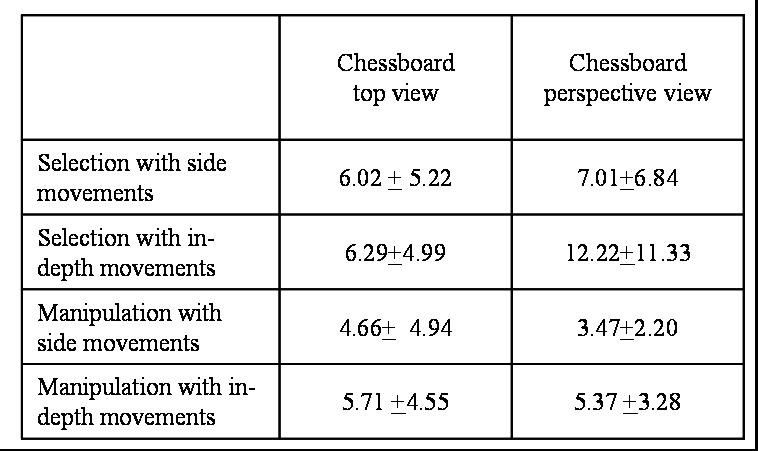
\includegraphics[width=.7\textwidth]{table.jpg}
\end{table}


\section{References}
\bibliographystyle{sbc}
\bibliography{sbc-template}

\end{document}

